\authoredsection{Chatbot Showcase Application}{Julius}{Julius Bethge}\label{sec:chatbot-application}

\subsection{Purpose and Design Rationale}\label{sec:application-purpose}

The pipeline components presented in the preceding chapter were integrated into a fully functioning showcase application. It provides one environment in which a user query can be routed, its trace inspected and evaluated, and resulting examples used for training or prompt optimization. The application was used by the project team, our Interhyp partners from the Data Science team, and is available to the supervisors from the LMU. It supported the development and evaluation of the pipeline as well as its demonstration within a fully functioning application. It is not an advisor-facing production system, a replacement for Robin, or a system already integrated into Interhyp's operational environment.

The application provided the project team and Interhyp with a shared environment for inspecting pipeline behavior, comparing configurations, and discussing potential integration. It can therefore be interpreted as a potential boundary object between technical development and stakeholder evaluation.\autocite{star-griesemer} This describes its intended role rather than an empirically tested organizational effect.

Validated approaches from the experimental \texttt{pipeline} repository were reimplemented in the maintainable \texttt{chatbot} showcase application.\autocite{amershi-ml-se}

Early integrations connected Python components through subprocesses and local files. Although functional, they lacked persistent shared state, coordination of long-running jobs, live progress, and lineage from a query through routing, answering, judging, and optimization. This confirmed that model code forms only one part of a complete machine-learning system.\autocite{sculley-technical-debt} We therefore retained a modular Python worker and added Convex for orchestration and persistence and React for presentation, preserving Python library access and replaceable providers while accelerating integration and deployment.

\subsection{Modular Architecture and Technology Rationale}\label{sec:application-architecture}

\subsubsection{Overall Architecture and Execution Flow}\label{sec:application-flow}

The architecture consists of a React frontend, Convex backend, and Python worker. Convex forms the shared state and orchestration layer. The frontend never calls the worker directly. This reflects the idea of a layered modular architecture in which components communicate through defined interfaces and can evolve or be recombined.\autocite{yoo-digital-innovation} Its specific realization with React, Convex, and Python is a project decision.

\begin{figure}
\centering
\pandocbounded{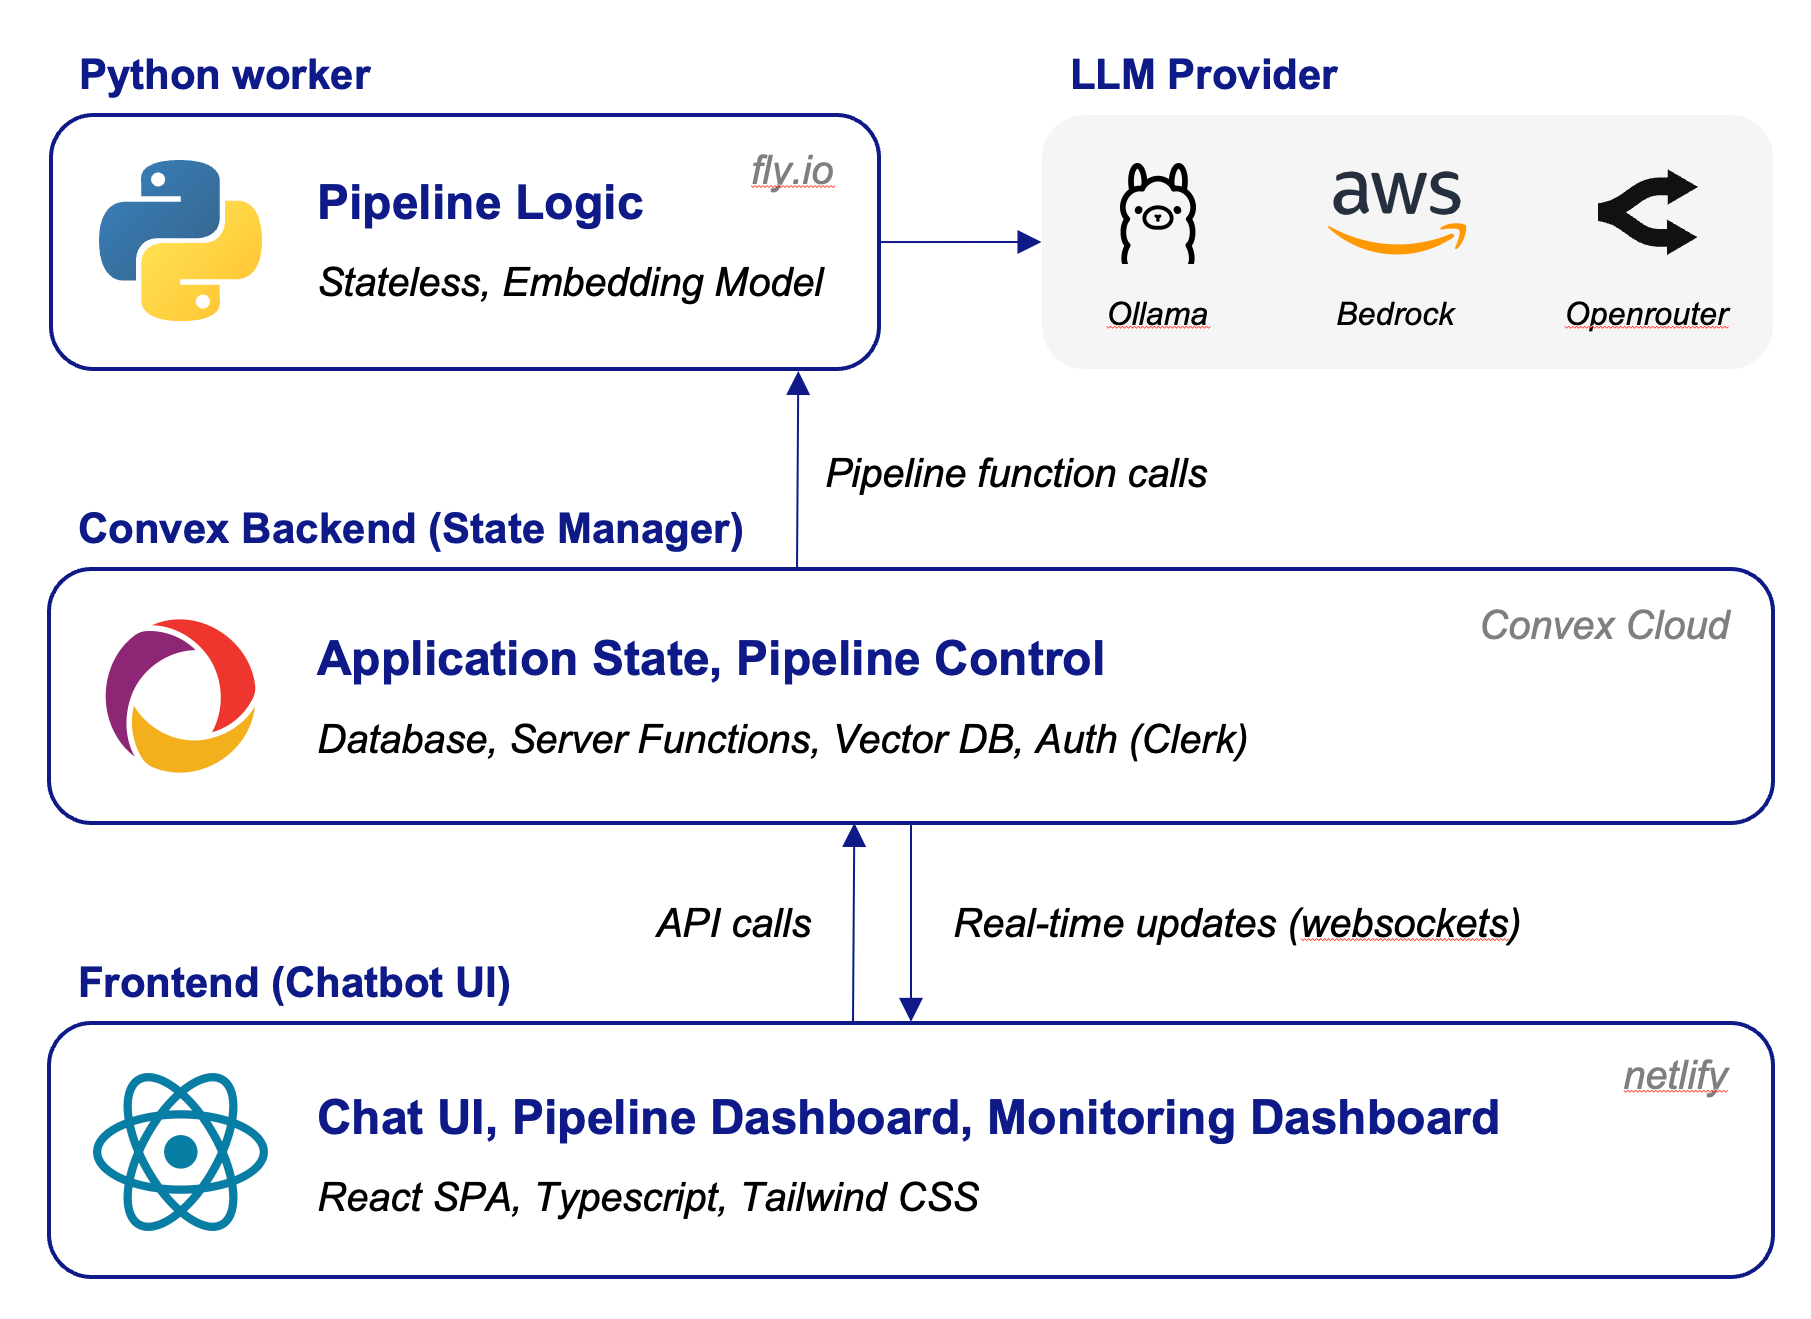
\includegraphics[keepaspectratio]{assets/application/architecture.png}}
\caption{Technical stack connecting the React frontend, Convex state layer, Python pipeline worker, and model providers}
\label{fig:application-architecture}
\end{figure}

Each operation is represented as a Convex job that the worker claims and updates with step statuses, inputs, outputs, errors, and timestamps before storing the resulting trace or run. Frontend subscriptions expose progress and preserve completed results across reloads, linking the same execution to the chatbot, pipeline, judge, training, and optimization views. Job states distinguish queued, running, successful, and failed executions, while step states also represent skipped conditional branches. The same protocol therefore supports interactive chat and longer batch or optimization runs without equating completion of a browser request with completion of the underlying computation.

\subsubsection{Python Worker}\label{sec:python-worker}

Python was retained because its machine-learning ecosystem provides the libraries and integrations required for embedding, model access, evaluation, and optimization.\autocite{raschka-python-ml} The worker owns all pipeline logic, including Stage 1 and Stage 2 routing, agent generation, judging, batch processing, index construction, and OPRO; Convex only schedules these operations and persists their state.

Provider interfaces decouple routing, completion, judging, optimization, and embedding from individual model services. Configuration selects execution mode, model identifiers, endpoints, timeouts, and credentials without changing the job protocol, trace model, or pipeline interfaces. Convex and React therefore form the showcase environment, while the worker remains reusable and could be adapted to Interhyp-approved endpoints. Such an integration was not performed.

This ownership boundary keeps embedding, routing, judging, and optimization decisions out of the backend and frontend. Either application layer could consequently be replaced without reconstructing pipeline rules.

\subsubsection{LLM and Embedding Provider Layer}\label{sec:provider-layer}

Stage 1 executes \texttt{multilingual-e5-large} inside the worker through FastEmbed's ONNX-based runtime and quantized weights.\autocite{fastembed-docs} The same setup is used locally and in the hosted application, avoiding changes in embedding behavior during integration. Computational efficiency also supported worker-local execution,\autocite{schwartz-green-ai} although a production deployment should compare it with a central embedding service when scaling workers.

Stage 2 requires token log probabilities, which OpenRouter exposes through \texttt{logprobs} and \texttt{top\_logprobs}.\autocite{openrouter-parameters} It therefore serves Stage 2 in the deployed configuration, while AWS Bedrock handles agent responses, judging, and OPRO using the available credits. Ollama remains the free local option but was too slow for some repeated and batch workflows. Because the hosted showcase cannot depend on a developer's computer, hosted mode uses OpenRouter and Bedrock, whereas local mode uses Ollama. The shared interfaces allow either configuration to be replaced with Interhyp-approved models.

\subsubsection{Convex Backend}\label{sec:convex-backend}

Convex forms the orchestration and state layer, storing jobs and steps, traces, prompt versions, vector entries, evaluation and training runs, and optimization history. Reactive queries expose worker progress without a separate WebSocket service or frontend polling,\autocite{convex-realtime} while schema-defined vector indexes support Stage 1 similarity search and retain links to source traces.\autocite{convex-vector-search} Generated TypeScript definitions connect backend functions with frontend queries and mutations.

Persistence makes lineage explicit through immutable prompt versions, a separately identified deployed version, run configurations, dataset snapshots, and traces linking queries to routing scores, agents, answers, timings, and judge outcomes. This extends model-management principles for retaining parameters, metrics, datasets, and historical changes.\autocite{vartak-modeldb} Reproducibility also requires accessible data, code, procedures, and execution conditions.\autocite{pineau-reproducibility} Storage alone cannot reproduce a result, but snapshots prevent later prompt or dataset changes from altering the basis of earlier runs and keep comparisons tied to identifiable conditions.

\subsubsection{React Frontend}\label{sec:react-frontend}

The React single-page frontend uses Vite, TypeScript, and Tailwind CSS to start workflows through Convex, subscribe to their state, and render live and completed executions across the chat, pipeline, evaluation, training, and optimization views. Shared components provide consistent statuses, selectors, scores, controls, and detail panels. Because Convex subscriptions expose worker updates as application state, the same components can display pending and completed executions without a second real-time channel. Public indexing and server rendering were unnecessary for the internal demonstrator.

\subsubsection{Authentication and Deployment}\label{sec:application-deployment}

Frontend and worker access follow separate authorization paths. Users authenticate through Clerk and Convex email and domain allowlists, whereas the Python worker supplies a shared token accepted only by worker-facing functions. A frontend session therefore cannot invoke worker operations, and the worker token grants no frontend access.

Netlify serves the React build, Convex Cloud hosts state, and Fly.io runs the containerized worker, with a Fly volume retaining the FastEmbed cache. Moving the frontend from Vercel to Netlify avoided a projected USD 300 cost, while Ollama remained available only for local development. These boundaries were sufficient for the controlled showcase; production integration would require Interhyp to evaluate service identity and secret management.

\subsection{Application Workflows and User Interface}\label{sec:application-workflows}

The interface supports individual chatbot execution, pipeline inspection, and evaluation, training, and optimization. Visible status, consistent controls, and inspectable results reflect Nielsen's usability principles.\autocite{nielsen-usability}

\subsubsection{Chatbot Interface}\label{sec:chatbot-interface}

Submitting a request creates a chat job whose routing summary and message area update during Stage 1, possible Stage 2 escalation, and agent generation. The completed view shows the answer, selected agent, routing stage, leading scores or probabilities, threshold, timings, and available vector or prompt references. Previous traces can be restored without another model call, connecting user-facing answers with their technical evidence.

Interactions are intentionally single-turn, limiting conversational state as a confounding factor and producing a stable evaluation unit containing the query, decision, answer, configuration, and timings. Each completed trace can be opened in the pipeline view or submitted to the judge.

\begin{figure}
\centering
\pandocbounded{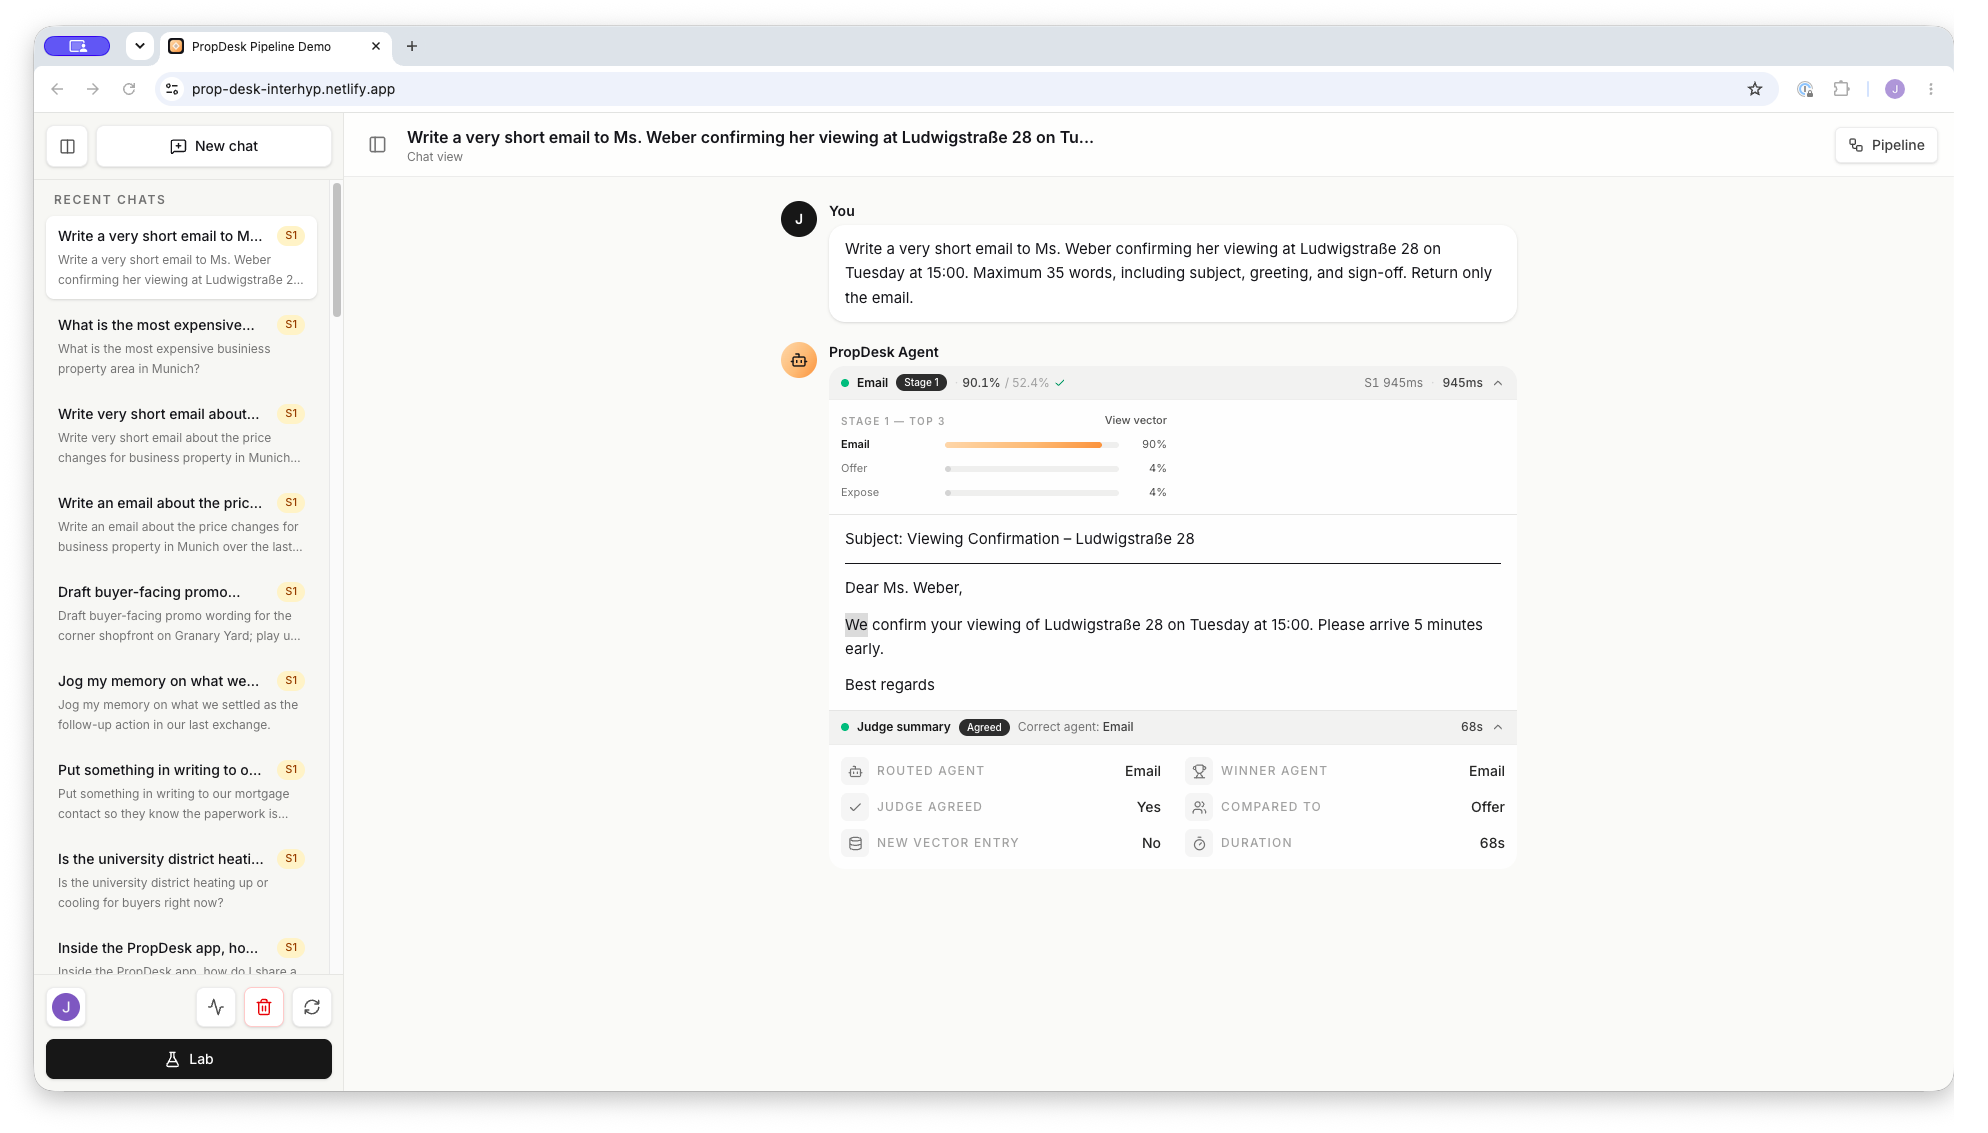
\includegraphics[keepaspectratio]{assets/application/chatbot-interface.png}}
\caption{Completed chatbot interaction with routing scores, trace history, and judge summary}
\label{fig:chatbot-interface}
\end{figure}

\subsubsection{Pipeline View}\label{sec:pipeline-view}

The pipeline view presents Router and judge execution as connected graphs. Nodes represent major steps and edges show their order and conditional paths. Pending, running, successful, skipped, and failed states change with the worker records. Stage 1 success follows a different visible path from Stage 2 escalation, and the judge pipeline becomes available for completed traces.

\begin{figure}
\centering
\pandocbounded{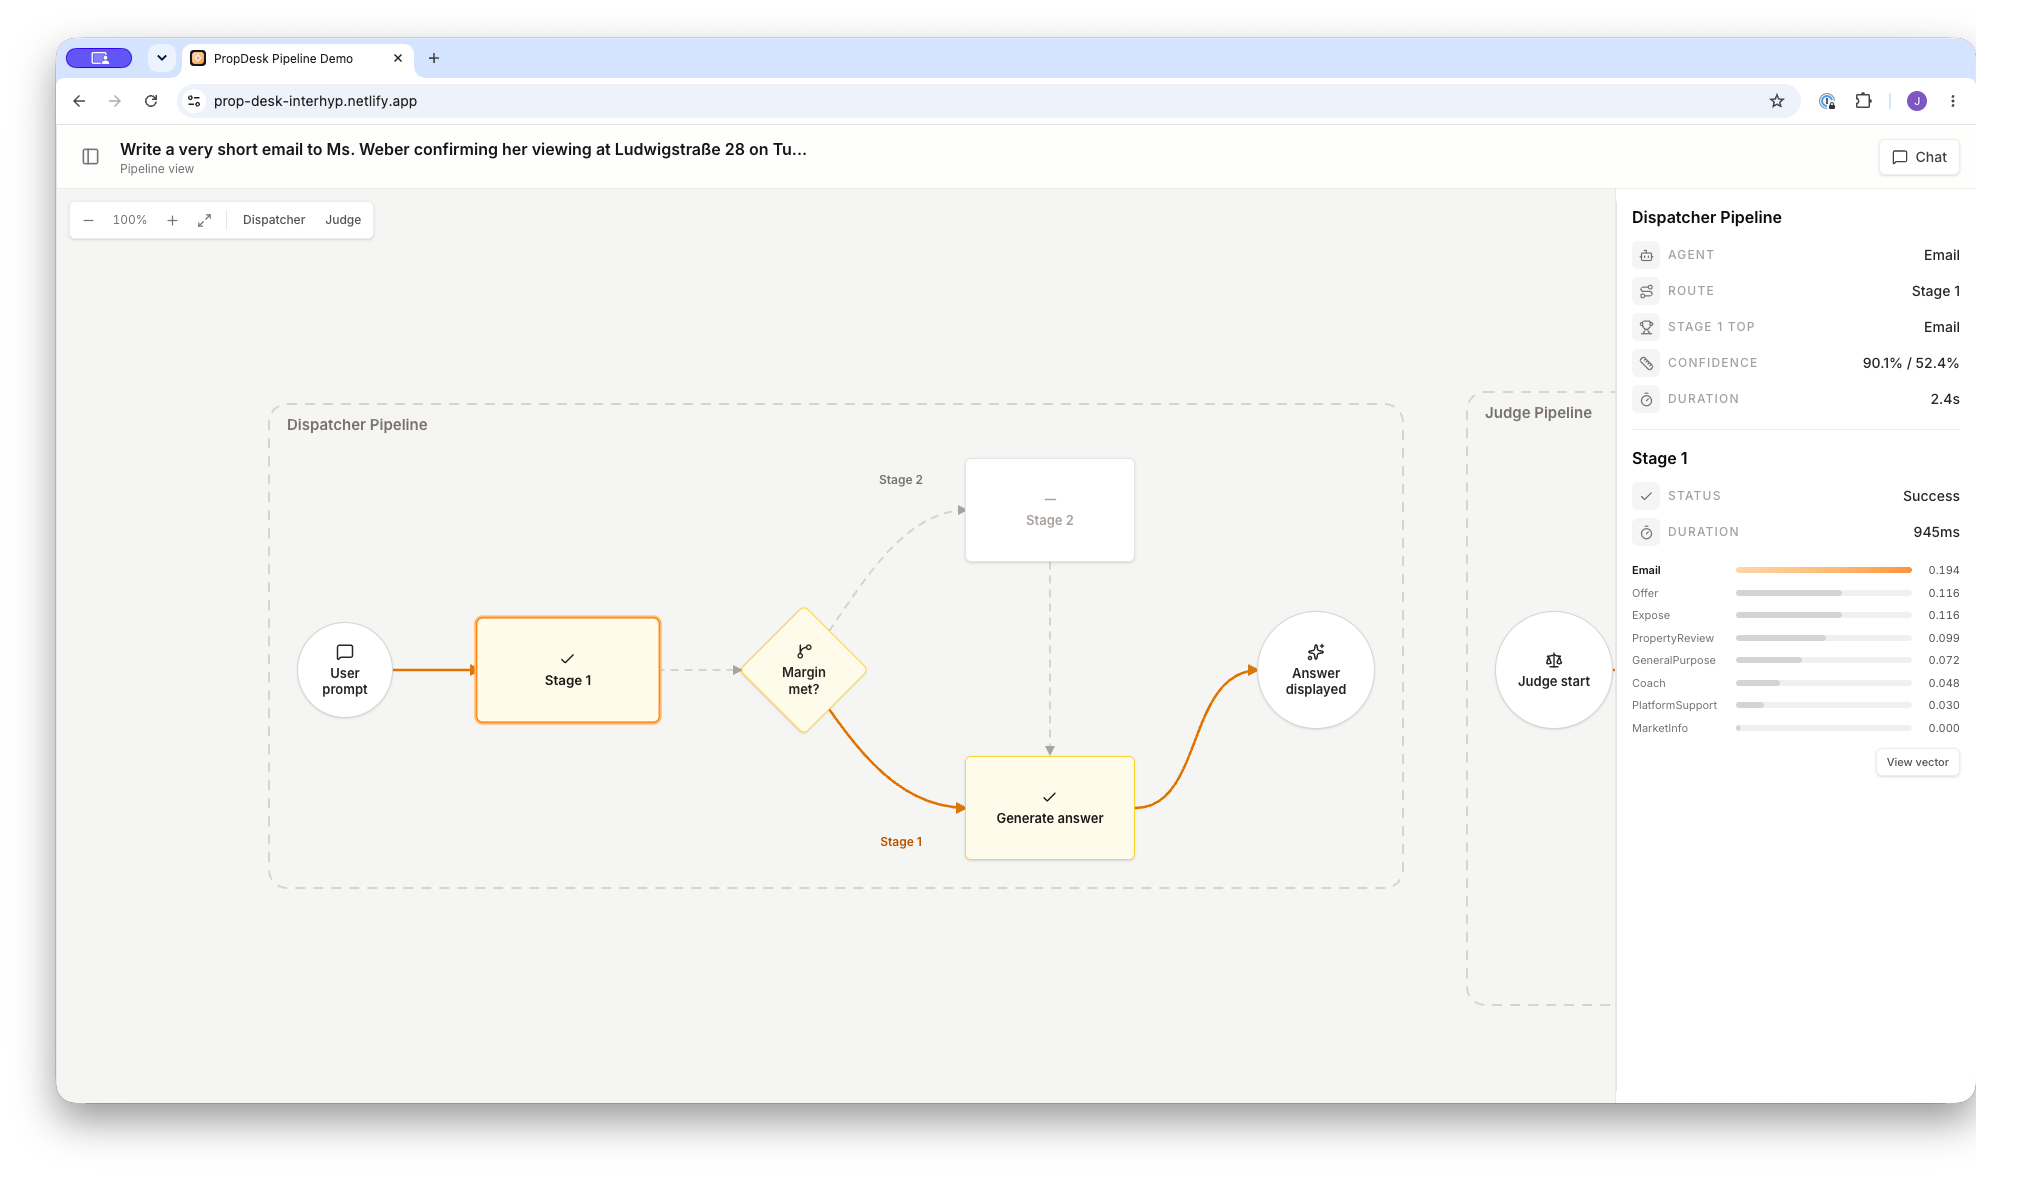
\includegraphics[keepaspectratio]{assets/application/router-pipeline.png}}
\caption{Router pipeline with the successful Stage 1 route and node inspector}
\label{fig:application-router-pipeline}
\end{figure}

Selecting a node opens an inspector with status, duration, inputs, outputs, scores, prompt or vector references, and stored payloads. This design applies Shneiderman's principle of providing an overview before details on demand.\autocite{shneiderman-eyes} It helps users understand an answer, locate unexpected execution and connect outcomes with intermediate evidence.

Conditional branches remain visible even when they are not executed, with their status distinguishing a skipped step from a failed one. This prevents a shortened Stage 1 path from appearing incomplete and makes Stage 2 escalation explicit. Router and judge diagrams share the same interaction pattern, so users can move from a high-level outcome to the evidence stored for a particular step without learning a separate inspection mechanism.

\begin{figure}
\centering
\pandocbounded{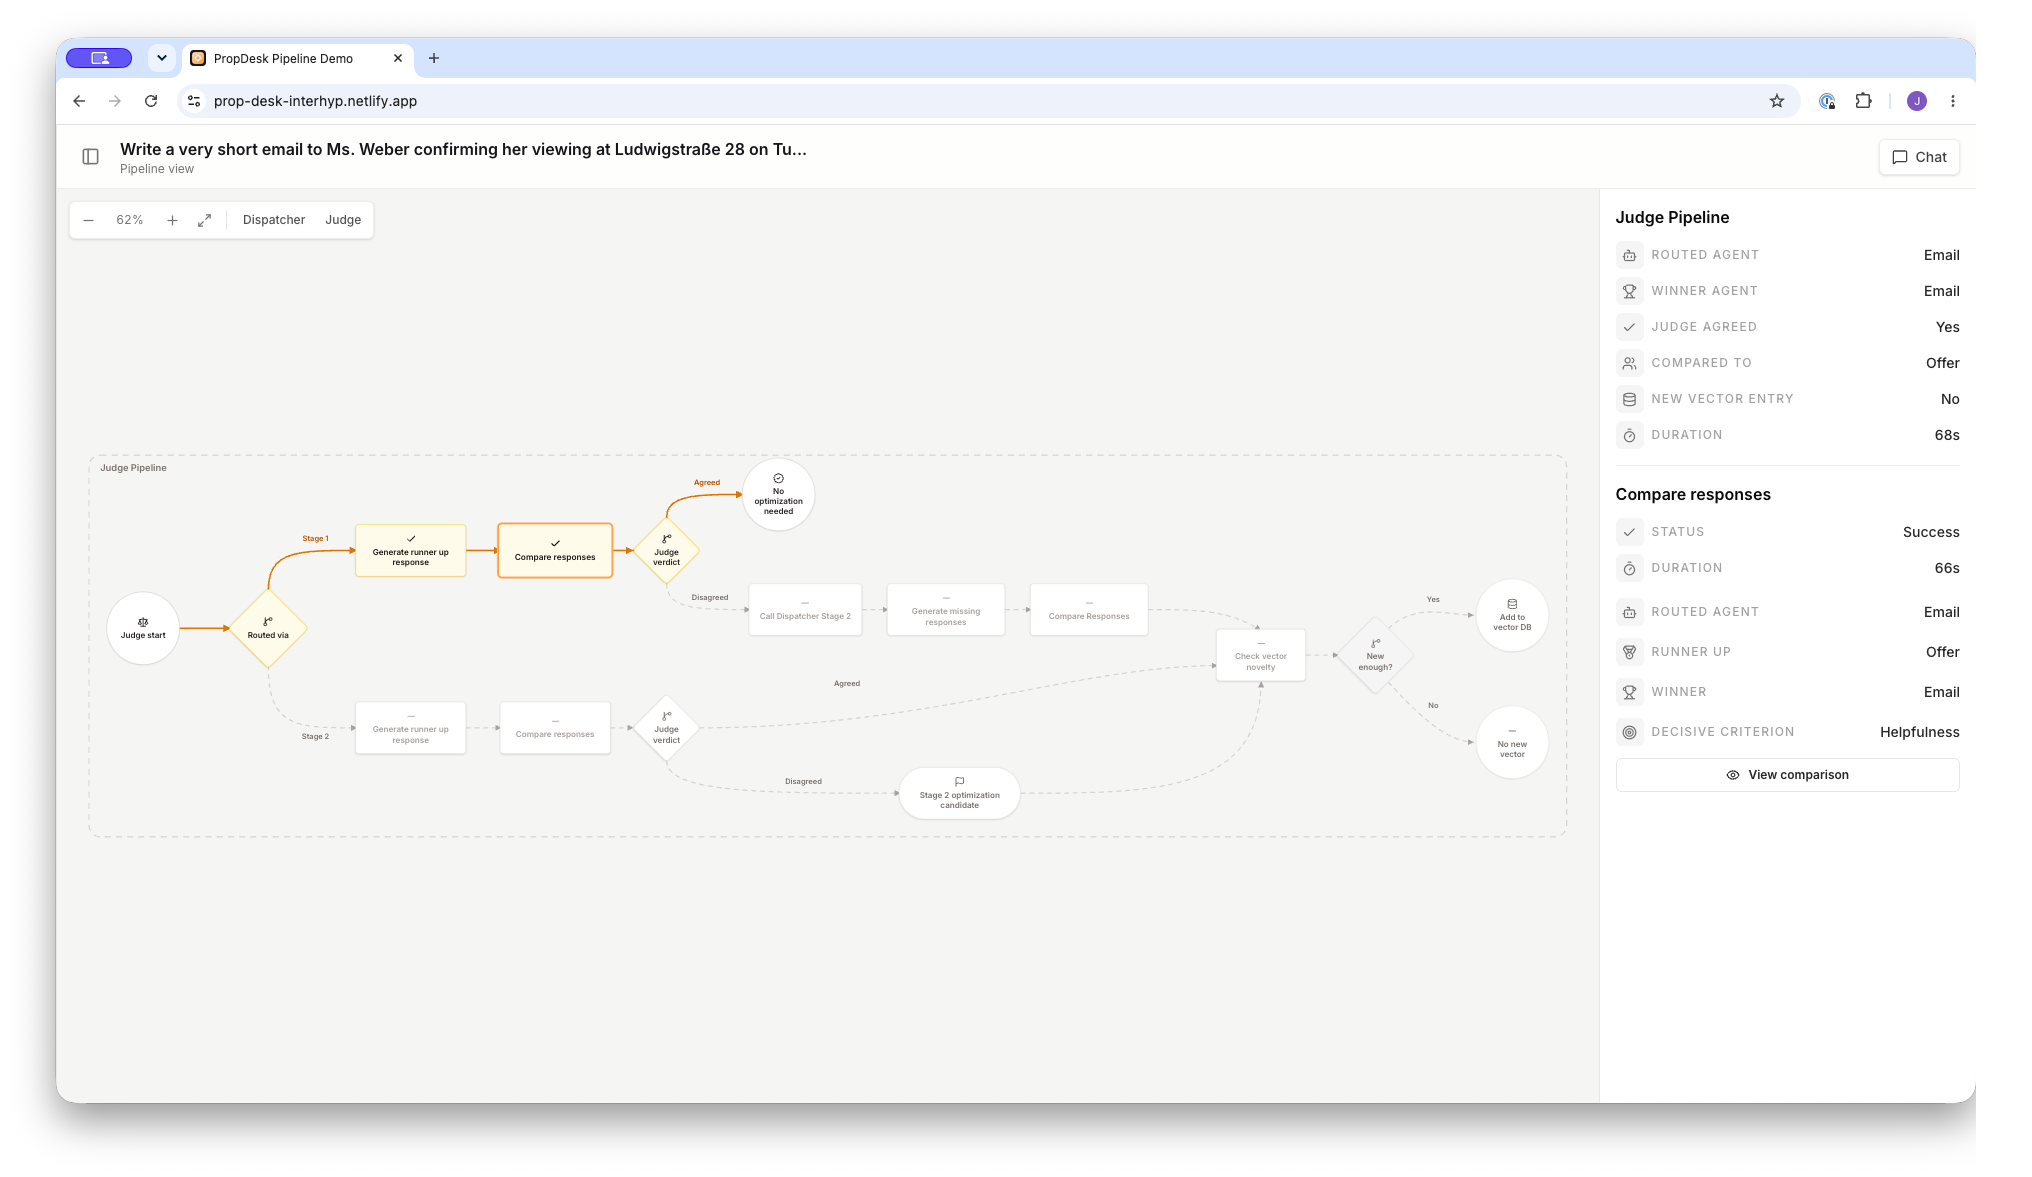
\includegraphics[keepaspectratio]{assets/application/judge-pipeline.png}}
\caption{Judge pipeline with the response-comparison step selected in the node inspector}
\label{fig:application-judge-pipeline}
\end{figure}

\subsubsection{Evaluation, Training and Optimization}\label{sec:evaluation-training-optimization}

The evaluation view runs a selected prompt version against the fixed evaluation dataset. Progress and individual outcomes remain visible during execution. Completed runs summarize accuracy, Stage 1 usage, latency, avoided LLM calls, misroutes, and per-agent results. Historical runs can be selected or compared while their prompt versions and configuration snapshots remain visible. A candidate can therefore be assessed under identifiable conditions before deployment.

\begin{figure}
\centering
\pandocbounded{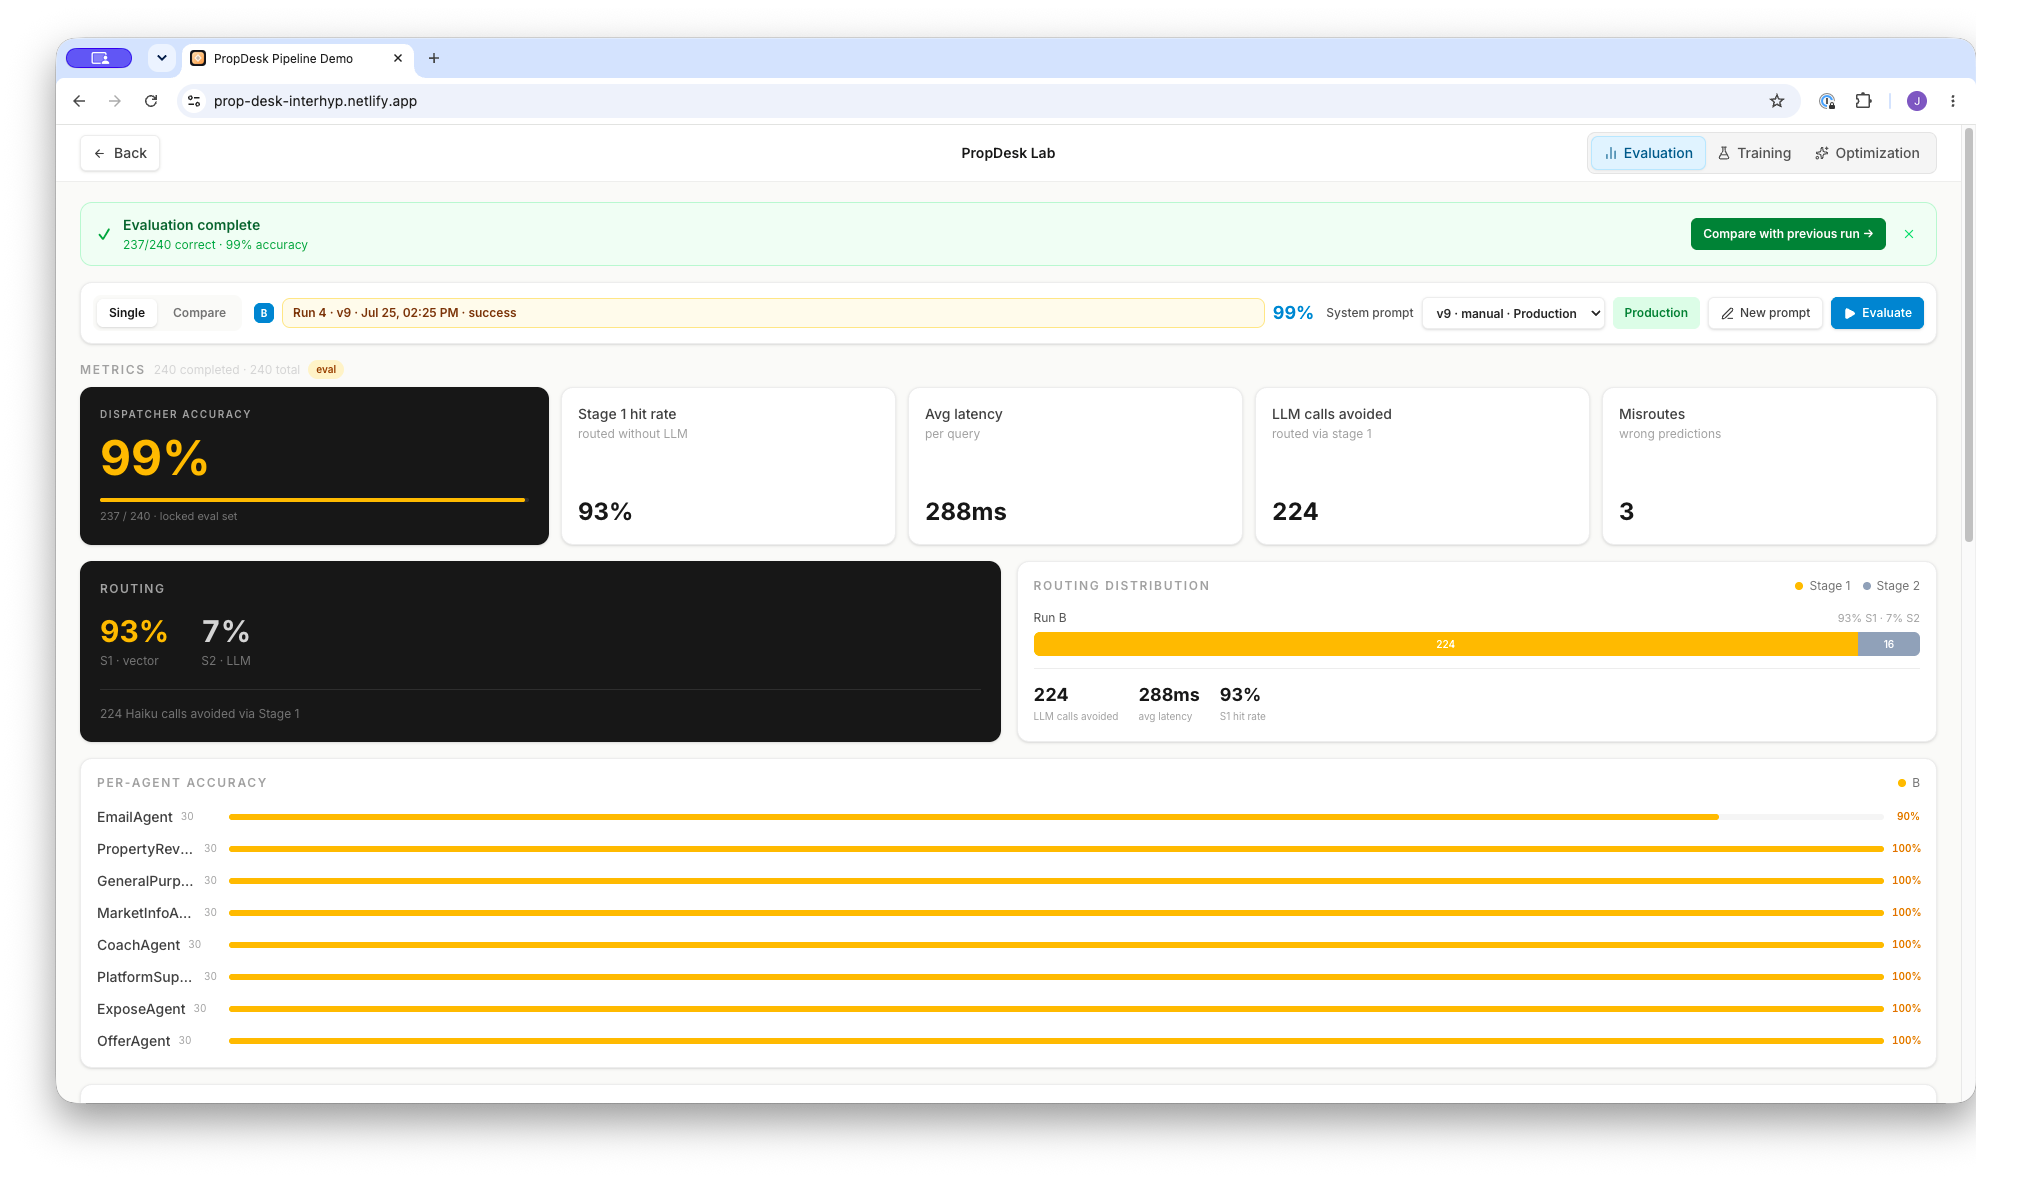
\includegraphics[keepaspectratio]{assets/application/evaluation-run.png}}
\caption{Completed evaluation run with routing, latency, and per-agent results}
\label{fig:application-evaluation}
\end{figure}

Training remains separate. Users upload labelled examples, and the application validates them and removes overlaps with the evaluation set. The resulting batch executes Router and judge workflows and records suitable Stage 1 corrections. A separate index-building job creates vector entries and threshold configuration while exposing its steps. This prevents evaluation examples from silently becoming training data.

\begin{figure}
\centering
\pandocbounded{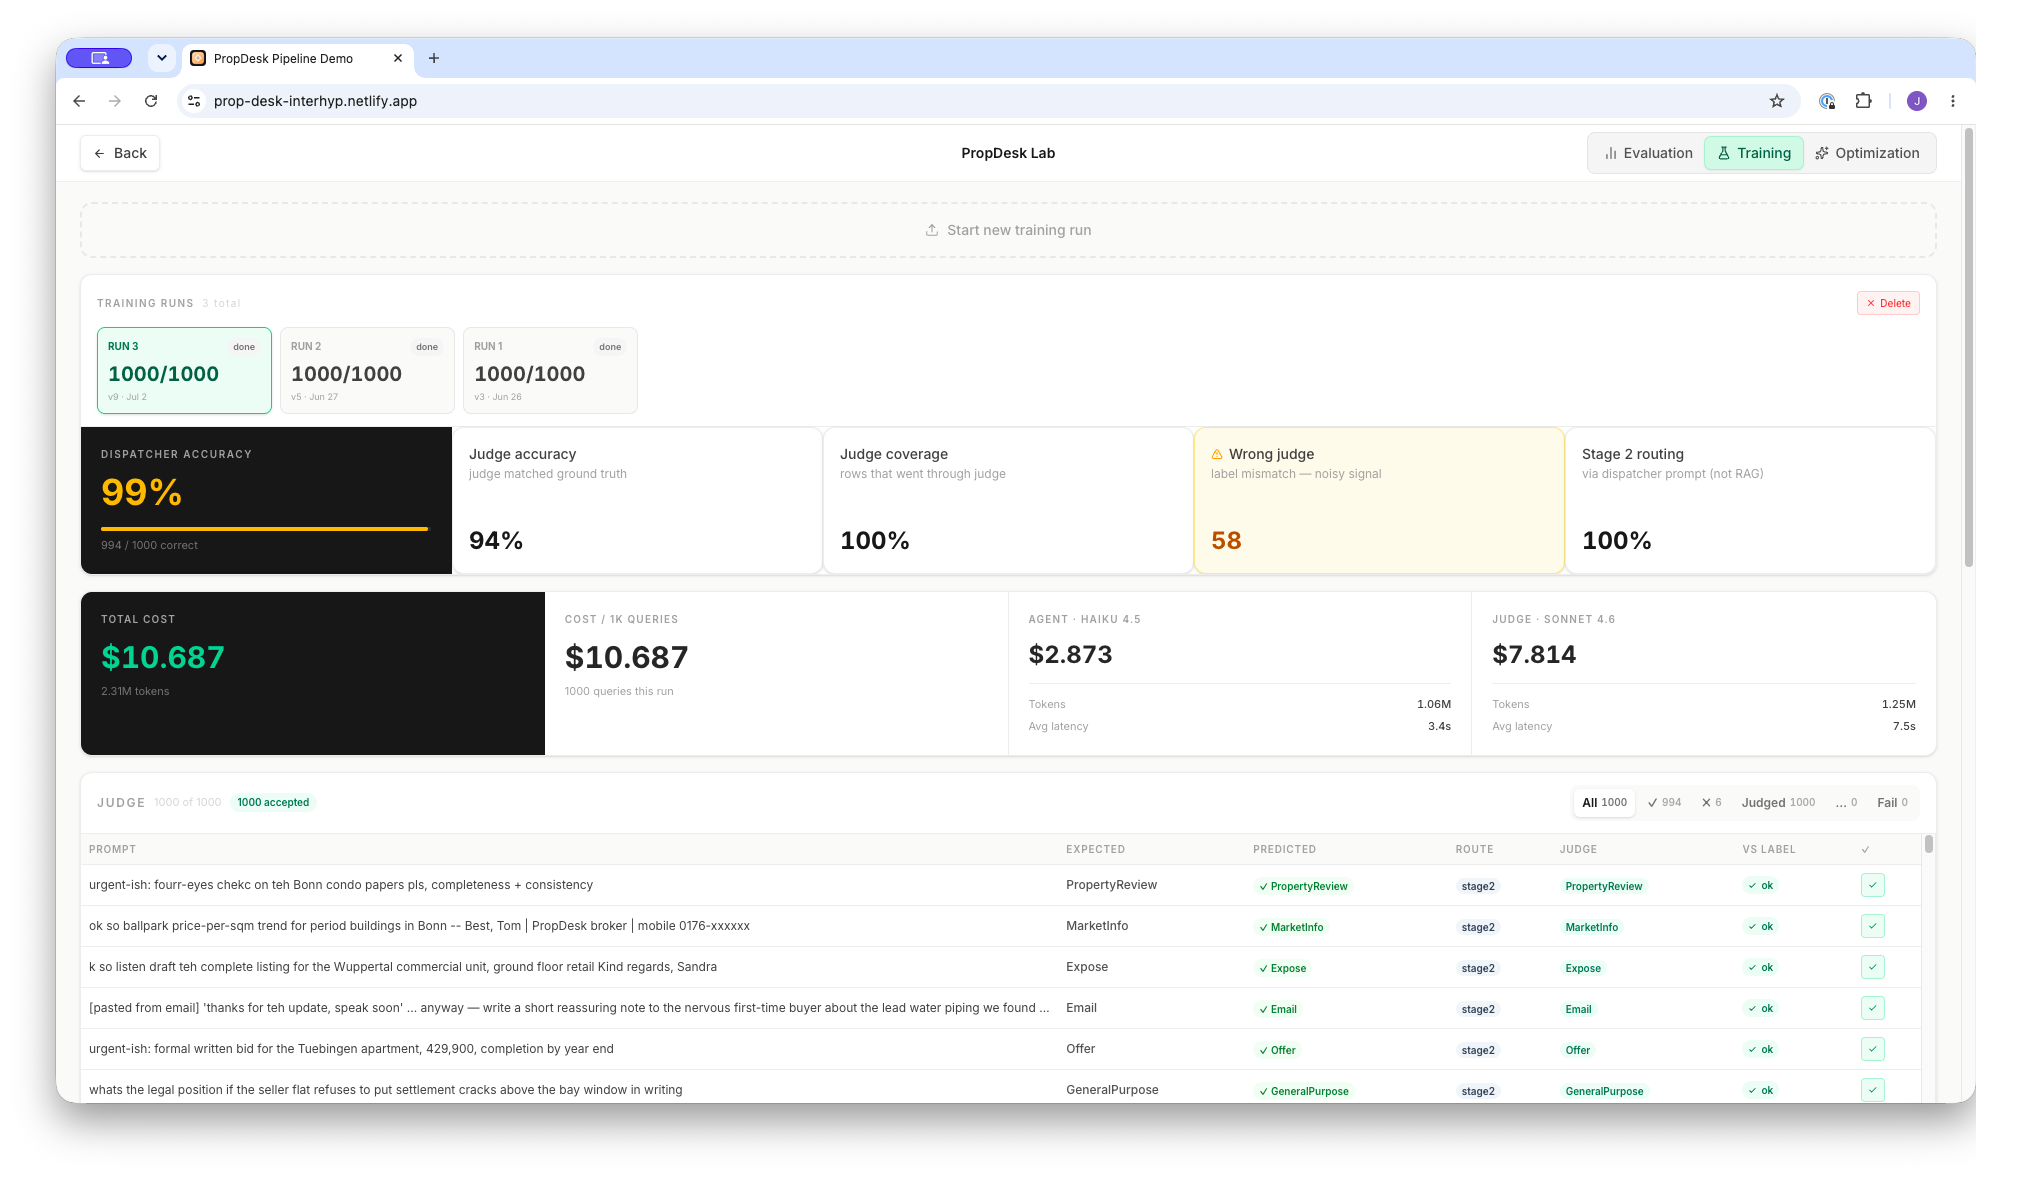
\includegraphics[keepaspectratio]{assets/application/training-run.png}}
\caption{Completed training run with routing, judge, cost, and trace-level results}
\label{fig:application-training}
\end{figure}

The optimization view applies OPRO to completed training data. Users follow rounds, candidate scores, and the optimization trajectory and can compare candidate prompts with the base prompt. Selecting a candidate creates a new prompt version. After evaluation, a version can be deployed without overwriting its predecessors.

\begin{figure}
\centering
\pandocbounded{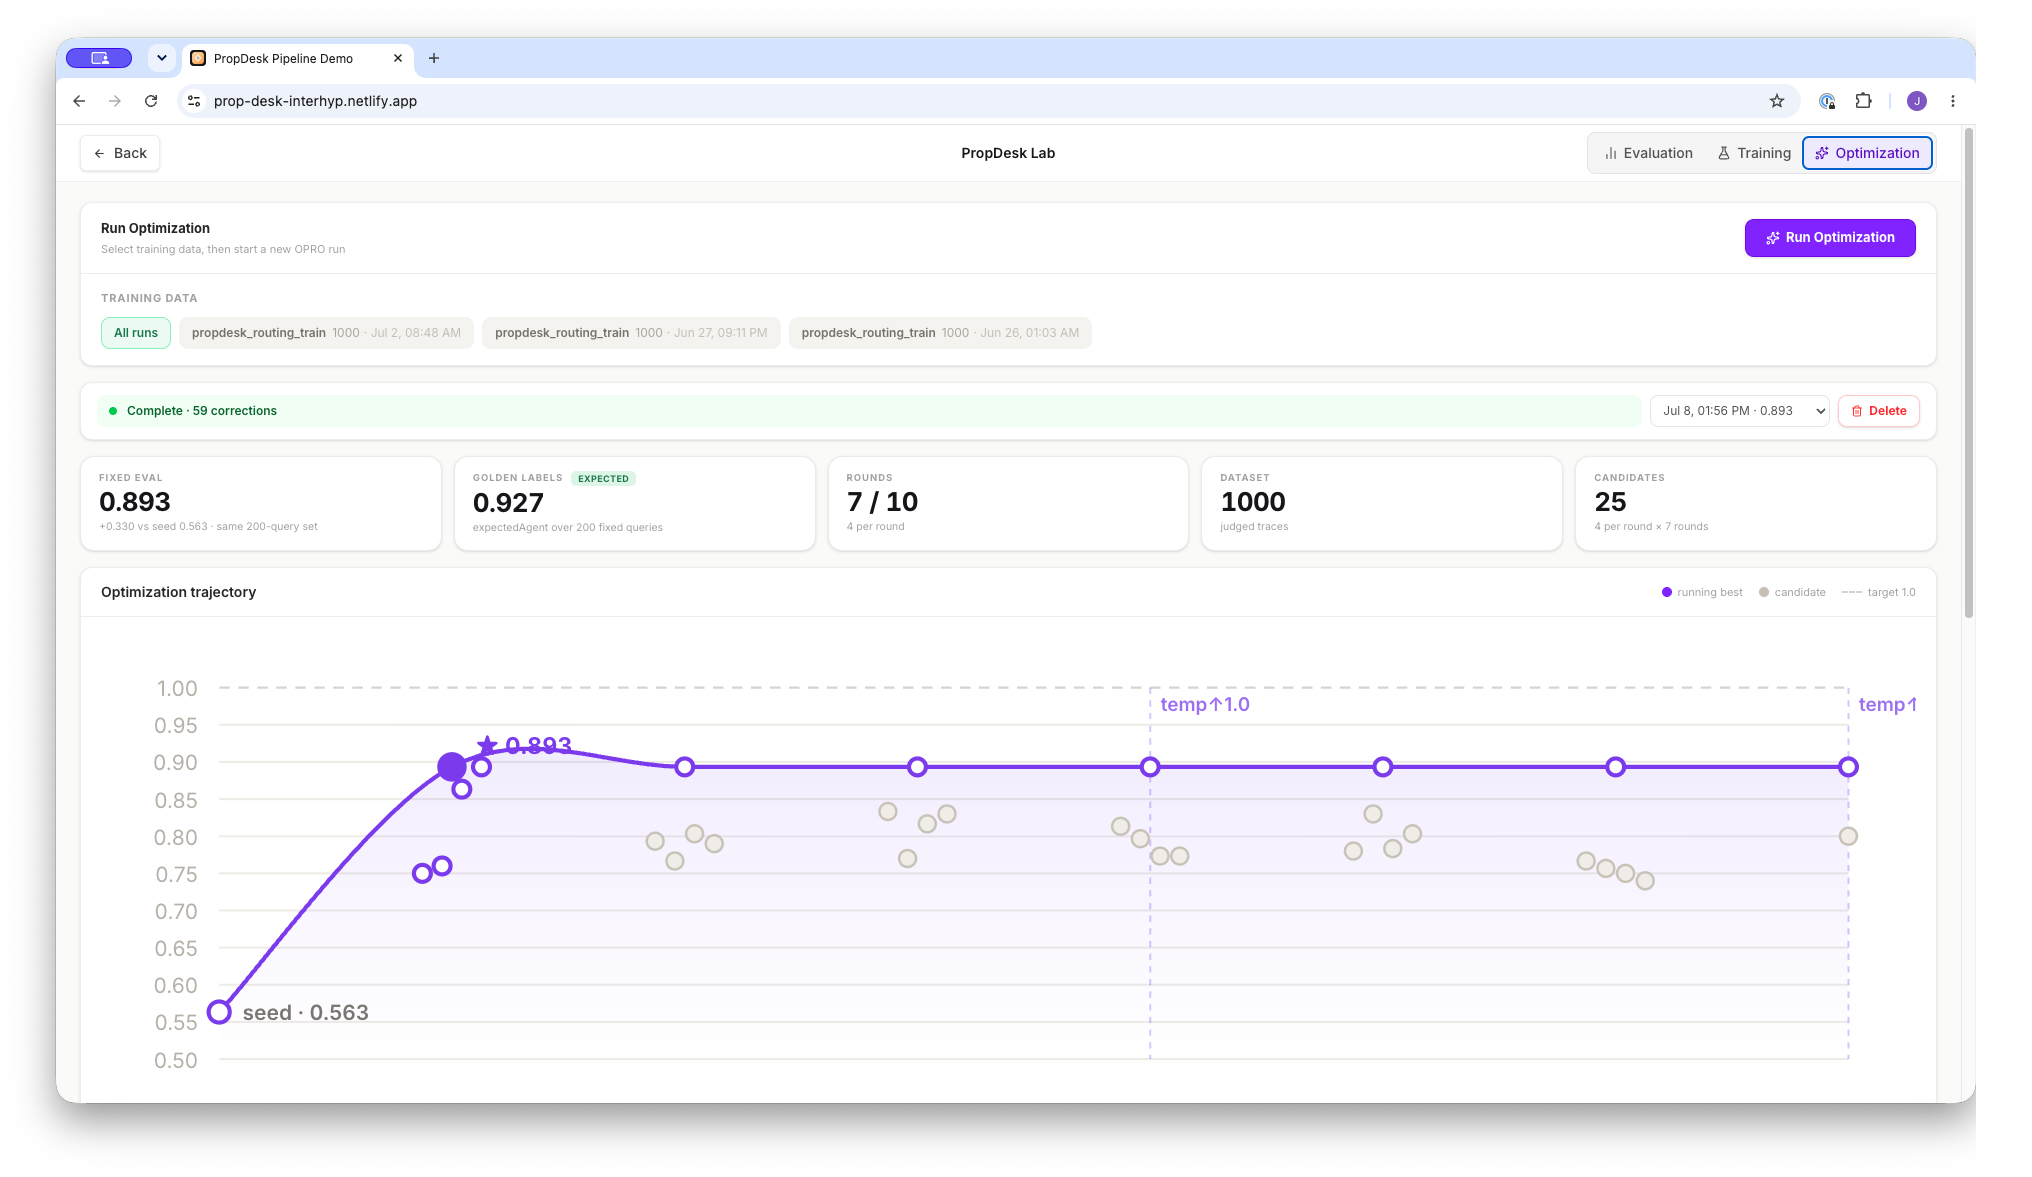
\includegraphics[keepaspectratio]{assets/application/optimization-run.png}}
\caption{Optimization trajectory showing the seed, candidate scores, and best fixed-evaluation result}
\label{fig:application-optimization}
\end{figure}

Together, the views create a traceable improvement cycle: training provides corrections and optimization inputs, optimization produces versioned candidates, and evaluation compares them on a fixed basis. Configuration snapshots, prompt lineage, and immutable run datasets allow users to move from aggregate results back to the runs and traces on which they depend.

The interface consequently distinguishes three actions that could otherwise be conflated. Evaluation measures a selected configuration without modifying the Stage 1 index. Training processes labelled examples and can contribute corrections to that index. Optimization searches for a stronger Stage 2 prompt but does not automatically replace the deployed version. Making these transitions explicit supports controlled experimentation and prevents a completed run from being mistaken for an automatically accepted system change.
